\chapter{2025}
\section*{一、程序阅读题}

1. 求以下代码的时间复杂度，并分析原因。

\begin{lstlisting}[language=C, basicstyle=\ttfamily]
void move(char a, char b, int n)
{
    printf("将第%d 个盘子从%c 移动到%c\n", n, a, b);
}

void F(int n, char a, char b, char c)
{
    if(n == 1)
        move(a, c, n);
    else
    {
        F(n-1, a, c, b);
        move(a, c, n);
        F(n-1, b, a, c);
    }
}
\end{lstlisting}

2. 下列代码交换双向链表中结点和结点的前驱。请填写完整代码。双向链表存储结构及功能函数如下：

\begin{lstlisting}[language=C, basicstyle=\ttfamily]
struct DLinkNode
{
    ElementType data;
    struct DLinkNode *prior;  // Front pointer
    struct DLinkNode *next;   // Rear pointer
};

void SwapWithPrevious(DLinkNode *p)
{
    DLinkNode *q = p->prior;
    ______①______;
    p->next = q;
    // 原回忆版中②在 q->prior=p 的后面,此处交换两者顺序
    ______②______;
    q->prior = p;
    p->prior->next = p;
    q->next->prior = q;
}
\end{lstlisting}

\newpage

3. 下列代码实现循环单链表队列的出队入队，请填写完整代码。队列的链式存储类型可以描述为：

\begin{lstlisting}[language=C, basicstyle=\ttfamily]
typedef struct LinkNode
{
    ElemType data;
    struct LinkNode *next;
} LinkNode;

typedef struct
{
    LinkNode *rear;
} LinkQueue;
\end{lstlisting}

入队出队操作函数如下：

\begin{lstlisting}[language=C, basicstyle=\ttfamily]
void EnQueue(LinkQueue *Q, LinkNode *p)
{
    if(Q->rear == NULL)
    {
        Q->rear = p;
        p->next = p;
    }
    else
    {
        ______①______;
        Q->rear->next = p;
        Q->rear = p;
    }
}

LinkNode* DeQueue(LinkQueue *Q)
{
    LinkNode *p;
    if(Q->rear == NULL)
        return NULL;
    p = Q->rear->next;
    if(Q->rear == p)
        ______②______;
    else
        Q->rear->next = p->next;
    return p;
}
\end{lstlisting}

4. 下列代码实现带头结点的单链表的简单选择排序，请填写完整代码。单链表存储结构如下：

\begin{lstlisting}[language=C, basicstyle=\ttfamily]
typedef struct LNode
{
    ElemType data;
    struct LNode *next;
} LNode, *LinkList;
\end{lstlisting}

选择排序功能函数如下：

\begin{lstlisting}[language=C, basicstyle=\ttfamily]
void SelectionSort(LinkList &L)
{
    LNode *p, *q, *min;
    ______①______;

    while(p != NULL)
    {
        min = p;
        q = p->next;

        while(q != NULL)
        {
            if(q->data < min->data)
                min = q;
            q = q->next;
        }

        if(______②______)
        {
            ElemType temp = p->data;
            p->data = min->data;
            min->data = temp;
        }
        ______③______;
    }
}
\end{lstlisting}

\section*{二、填空题}

5. 分析这段代码在给定输入 a[] = \{5,4,3,2,1\} 的时间复杂度为\_\_\_\_\_\_\_\_\_\_。

\begin{lstlisting}[language=C, basicstyle=\ttfamily]
void F(int a[], int i, int n)
{
    if(i >= n-1)
        return;
    // 不是冒泡排序,若要修改,则修改成注释循环部分
    // for(int j=0; j<n-1-i; j++)
    for(int j=i; j<n-1; j++)
    {
        if(a[j] > a[j+1])
        {
            int temp = a[j];
            a[j] = a[j+1];
            a[j+1] = temp;
        }
    }
    F(a, i+1, n);
}
\end{lstlisting}

6. 元素 1,1,2,3,4 依次入栈，以 4 为开头的出栈序列有\_\_\_\_\_\_\_\_\_\_个。

7. 已知数组 \(A_{9\times 3\times 5\times 8}\)，其中 A[0][0][0][0] 的地址为 100，每一个整数占 4B，则 A[2][1][4][7] 的地址为\_\_\_\_\_\_\_\_\_\_。

8. 哈夫曼树有 199 个结点，则叶子结点有\_\_\_\_\_\_\_\_\_\_个。

9. 对于后缀表达式 1 2 4 2 / + 5 * -，经过运算后的值为\_\_\_\_\_\_\_\_\_\_。

10. 森林 F 有 15 条边，25 个结点，则森林中一共有\_\_\_\_\_\_\_\_\_\_棵树。

11. 设广义表 L = ((a,b),(c,d))，求 getHead(getTail(L)) = \_\_\_\_\_\_\_\_\_\_。

12. 利用 KMP 算法，求 abcaaba 的 next 数组\_\_\_\_\_\_\_\_\_\_。

13. 在一棵度为 4 的树 T 中，若有 20 个度为 4 的结点，10 个度为 3 的结点，1 个度为 2 的结点，10 个度为 1 的结点，则树中叶节点的个数为\_\_\_\_\_\_\_\_\_\_。

14. 如图所示，有一个小根堆，当插入后，小根堆经过调整后为\_\_\_\_\_\_\_\_\_\_。

\begin{figure}[htbp]
    \centering
    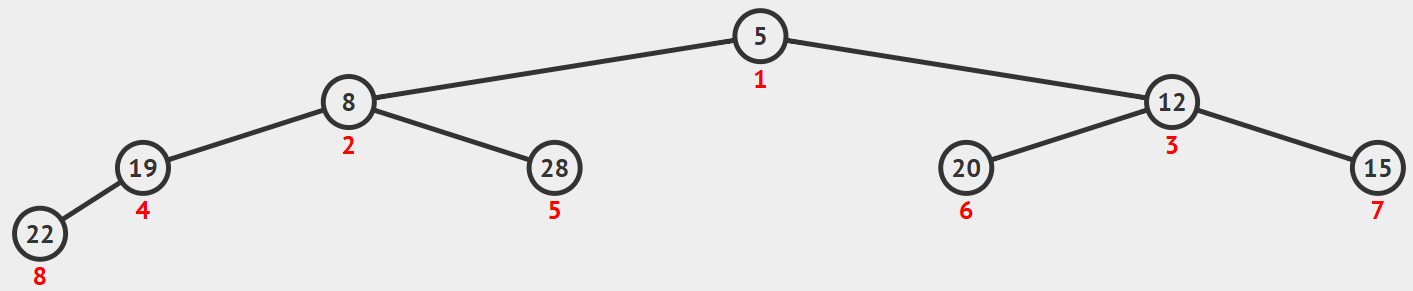
\includegraphics[width=0.3\textwidth]{images/2025/blank_14.png}
    \caption*{图1 14题图}
\end{figure}

\section*{三、综合应用题}

15. 已知一棵二叉查找树/二叉排序树(BST)的先序遍历序列为 23,15,12,18,56,29,34,71。

(1) 请画出此二叉树的形态；

(2) 请给出这棵树的后序遍历序列；

(3) 画出此二叉树的中序线索二叉树；

(4) 画出与此二叉树对应的森林。

\vspace{10em}

16. 设散列表为 HT[0...12]，即表的大小为 m=13。现采用双散列法解决冲突。散列函数和再散列函数分别为：

\[
H_{0}(key) = key \bmod 13
\]

\[
H_{i} = (H_{i-1} + (\mathrm{reverse}(key) + 1) \bmod 11 + 1) \bmod 13
\]

其中 reverse(x) 是将 x 逆置，如：reverse(789)=987。

(1) 若输入的关键码为 2,8,31,20,70,59,25,28，请画出插入这 8 个关键码后得到的散列表。

(2) 计算查找成功的平均查找长度 ASL。

\vspace{10em}

\newpage

17. 给定字符 a 到 g，它们的权值分别如下：

a:5, b:9, c:12, d:13, e:16, f:45, g:50

(1) 请根据给定的字符及其对应的权值，使用哈夫曼编码算法构建一棵哈夫曼树。要求在每次合并两个结点时，确保左结点的权值小于等于右结点的权值。

(2) 根据哈夫曼树的结构，写出每个字符的哈夫曼编码，要求左结点为 0，右结点为 1，填出下表中的对应编码。

\begin{figure}[htbp]
    \centering
    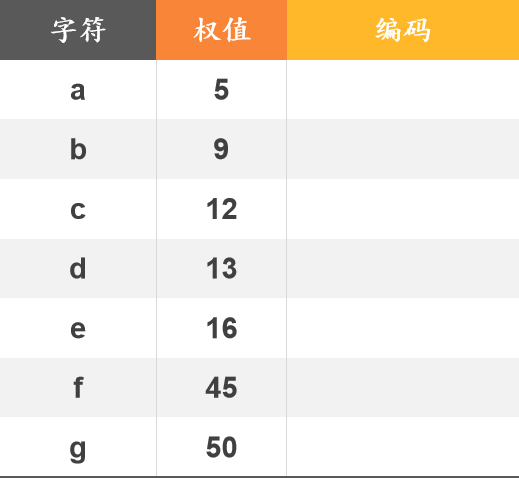
\includegraphics[width=0.3\textwidth]{images/2025/comprehensive_17.png}
    \caption*{图2 17题图}
\end{figure}

18. 已知有序数组为 [7,15,23,35,41,53,62,70,81,94]，对该数组进行二分查找，回答下列问题：

(1) 画出二叉查找树；

(2) 查找 53 需要找哪些元素；

(3) 查找 90 需要找哪些元素；

(4) 计算查找成功和查找失败的平均查找长度。

\vspace{10em}

\newpage

19. 已知带权的完全无向图 G，回答以下问题：

(1) 从 A 开始，分别写出图 G 的广度优先搜索(BFS)和深度优先搜索(DFS)序列。如果在遍历过程中有多个相同权值的路径，优先选择字母顺序较小的结点；

(2) 使用 Prim 算法从结点 A 开始构建最小生成树。如果在选择路径时存在多个相同权值的路径，优先选择字母顺序较小的结点；

(3) 使用 Kruskal 算法构建最小生成树。如果在选择路径时存在多个相同权值的路径，优先选择字母顺序较小的结点。

\begin{figure}[htbp]
    \centering
    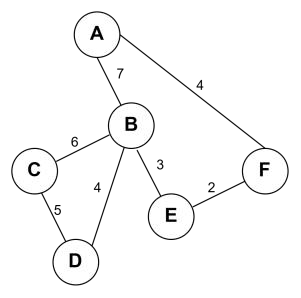
\includegraphics[width=0.3\textwidth]{images/2025/comprehensive_19.png}
    \caption*{图3 19题图}
\end{figure}

20. 给定一个 AOE 网，请回答以下问题：

(1) 计算每个事件的最早发生时间(\(ve\))和最晚发生时间(\(vl\))；

(2) 计算每个活动的最早开始时间(\(e\))和最迟开始时间(\(l\))；

(3) 确定关键路径。

\begin{figure}[htbp]
    \centering
    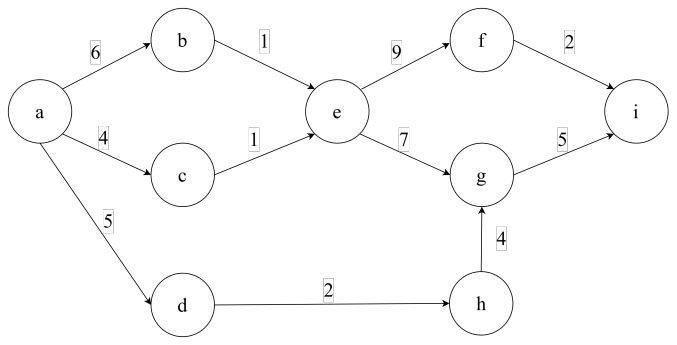
\includegraphics[width=0.3\textwidth]{images/2025/comprehensive_20.png}
    \caption*{图4 20题图}
\end{figure}

\newpage

\section*{四、算法设计与分析题}

21. 给定一个单链表，找到倒数第 k 个元素。如果找到该元素，打印该元素的值并返回 1，否则返回 0。

(1) 描述算法的基本设计思想；

(2) 根据设计思想，采用 C 语言描述算法。

结点定义如下：

\begin{lstlisting}[language=C, basicstyle=\ttfamily]
typedef struct node
{
    int data;
    struct node *next;
} LNode, *LinkList;
\end{lstlisting}

\vspace{15em}

\newpage

22. 给定一棵二叉树，输出从根结点到叶子结点的最长路径，打印路径的结点值，并输出该路径的长度。

(1) 描述算法的基本设计思想；

(2) 根据设计思想，采用 C 语言描述算法。

二叉树的链式存储结构描述如下：

\begin{lstlisting}[language=C, basicstyle=\ttfamily]
typedef struct BiTNode {
    ElemType data;
    struct BiTNode *lchild, *rchild;
} BiTNode, *BiTree;
\end{lstlisting}

\vspace{15em}

\newpage

23. 给定一个邻接表表示的连通图，输出从顶点 \(u\) 到顶点 \(v\) 并经过顶点 \(k\) 的一条路径。如果不存在这样的路径，输出 -1。

(1) 描述算法的基本设计思想；

(2) 根据设计思想，采用 C 语言描述算法。

图的存储结构描述如下：

\begin{lstlisting}[language=C, basicstyle=\ttfamily]
#define MaxVertexNum 100
typedef char InfoType;   // 附加信息类型
typedef int VertexType;  // 顶点数据类型

typedef struct ArcNode {  // 边表结点
    int adjvex;           // 该弧所指向的顶点位置
    struct ArcNode *next; // 下个结点
    // InfoType info;     // 当前结点（弧）的信息
} ArcNode;

typedef struct VNode {        // 顶点表结点
    VertexType data;          // 顶点信息
    ArcNode *firstarc;        // 指向第一条依附该顶点的弧的指针
} VNode, AdjList[MaxVertexNum];

typedef struct {              // 图
    AdjList vertices;         // 邻接表
    int vexnum, arcnum;       // 图的当前顶点数,图的边数/弧数
} ALGraph;
\end{lstlisting}
